\documentclass[usenames,dvipsnames,aspectratio=169]{beamer}
\usepackage{../common/prg}

\title[8. előadás]{Programozás}
\subtitle{(GKxB\_INTM114)}

\begin{document}

%1
\begin{frame}[plain]
  \titlepage
  \logoalul
\end{frame}

%2
\section{Dinamikus memóriakezelés}
\subsection{A tömbök rugalmatlanok}
\begin{frame}
  Feladat:
  \begin{itemize}
    \item Fejlesszük tovább úgy a buborék rendezőalgoritmust bemutató példát, hogy a felhasználó adhassa meg a rendezendő adatokat! (Adatbevitelnek vége negatív adatra.)
    \item Nem adhat meg több számot, mint a tömb elemszáma!
  \end{itemize}
  \vfill
  Problémák:
  \begin{itemize}
    \item Fordítási időben tudni kellene a rendezendő adatok számát
    \item Túl kicsi tömb $\to$ nem férnek el az adatok
    \item Túl nagy tömb $\to$ pazaroljuk a memóriát
    \item Inkább nagyobb legyen a tömb, mint túl kicsi!
  \end{itemize}
\end{frame}

%3
\begin{frame}[fragile]
  \begin{columns}[T]
    \column{0.47\linewidth}
      \begin{block}{Kimenet -- leállás végjelre}
        \begin{verbatim}
Adjon meg nemnegativ szamokat!
1. szam: 2
2. szam: 4
3. szam: 1
4. szam: 3
5. szam: -1
Rendezes utan:
1       2       3       4       
        \end{verbatim}
      \end{block}
    \column{0.47\linewidth}
      \begin{block}{Kimenet -- leáll amikor a tömb megtelik}
        \begin{verbatim}
Adjon meg nemnegativ szamokat!
1. szam: 5
2. szam: 4
3. szam: 3
4. szam: 2
5. szam: 1
Rendezes utan:
1       2       3       4       5       
        \end{verbatim}
      \end{block}
  \end{columns}
\end{frame}

%4
\begin{frame}
  \begin{exampleblock}{\textattachfile{buborek5.cpp}{buborek5.cpp}}
    \vspace{-0.2cm}
    \lstinputlisting[style=cpp,linerange={3-3},numbers=left,firstnumber=3]{buborek5.cpp}
    \lstinputlisting[style=cpp,linerange={37-46},numbers=left,firstnumber=37]{buborek5.cpp}
    \vspace{-0.2cm}
  \end{exampleblock}
\end{frame}

%5
\begin{frame}
  \begin{exampleblock}{\textattachfile{buborek5.cpp}{buborek5.cpp}}
    \vspace{-0.2cm}
    \lstinputlisting[style=cpp,linerange={5-16},numbers=left,firstnumber=5]{buborek5.cpp}
    \vspace{-0.2cm}
  \end{exampleblock}
\end{frame}

%6
\subsection{Futásidejű memóriafoglalás és -felszabadítás, memóriamenedzsment}
\begin{frame}
  Dinamikus memóriakezelés
  \begin{itemize}
    \item A programozó dönt a dinamikus változók élettartamáról
    \item Memória foglalás:
    \begin{description}[mmm]
      \item[C++] \texttt{new} operátorral $\to$ megfelelő típusú mutatót ad vissza, nincs szükség típuskényszerítésre
      \item[C] \texttt{\hiv{\href{https://en.cppreference.com/w/c/memory/malloc}{malloc()}}}, \texttt{\hiv{\href{https://en.cppreference.com/w/c/memory/calloc}{calloc()}}} függvények, \texttt{void*} mutatóval térnek vissza
    \end{description}
    \item Terület felszabadítása:
    \begin{description}[mmm]
      \item[C++] \texttt{delete} operátorral
      \item[C] \texttt{\hiv{\href{https://en.cppreference.com/w/c/memory/free}{free()}}} függvénnyel
      \item[\usebeamertemplate{itemize item}] Ugyanaz a terület nem szabadítható fel többször
      \item[\usebeamertemplate{itemize item}] NULL/nullptr mutató felszabadítása nem okoz gondot  
    \end{description}
  \end{itemize}
\end{frame}

%7
\subsection{Futásidejű memóriafoglalás és -felszabadítás, inicializáció}
\begin{frame}
  \begin{itemize}
    \item Foglalt terület átméretezése:
    \begin{description}[mmm]
      \item[C++] nincs eszköz, a problémát specifikus osztály(sablon)okkal kerülik el, pl. \texttt{\hiv{\href{https://en.cppreference.com/w/cpp/string/basic\_string}{std::string}}}, \texttt{\hiv{\href{https://en.cppreference.com/w/cpp/container/vector}{std::vector}}} $\to$ következő félév anyaga
      \item[C] \texttt{\hiv{\href{https://en.cppreference.com/w/c/memory/realloc}{realloc()}}}
    \end{description}
    \item A C/C++ memóriakezelő megoldásai nem keverhetők egymással (pl. memóriafoglalás \texttt{new}-val majd \texttt{realloc()})
  \end{itemize}
\end{frame}

%8
\begin{frame}
  \begin{exampleblock}{\textattachfile{dinamikus1.cpp}{dinamikus1.cpp}}
    \lstinputlisting[style=cpp,linerange={5-11},numbers=left,firstnumber=5]{dinamikus1.cpp}
  \end{exampleblock}
\end{frame}

%9
\begin{frame}
  \begin{exampleblock}{\textattachfile{dinamikus1.cpp}{dinamikus1.cpp}}
    \vspace{-0.2cm}
    \small
    \lstinputlisting[style=cpp,linerange={13-19},numbers=left,firstnumber=13]{dinamikus1.cpp}
    \vspace{-0.2cm}
  \end{exampleblock}
  \begin{exampleblock}{\textattachfile{dinamikus2.cpp}{dinamikus2.cpp} -- A lefoglalt terület inicializálható}
    \vspace{-0.2cm}
    \small
    \lstinputlisting[style=cpp,linerange={9-11},numbers=left,firstnumber=9]{dinamikus2.cpp}
    \vspace{-0.2cm}
  \end{exampleblock}
\end{frame}

%10
\begin{frame}
  Struktúráknak is foglalható memória dinamikusan, amit akár inicializáció is követhet
  \begin{exampleblock}{\textattachfile{dinamikus3.cpp}{dinamikus3.cpp}}
    \footnotesize
    \vspace{-0.2cm}
    \lstinputlisting[style=cpp,linerange={4-7},numbers=left,firstnumber=4]{dinamikus3.cpp}
    \lstinputlisting[style=cpp,linerange={10-17},numbers=left,firstnumber=10]{dinamikus3.cpp}
    \vspace{-0.2cm}
  \end{exampleblock}
\end{frame}

%11
\begin{frame}
  Tömböknek is lehet dinamikusan memóriát foglalni
  \begin{exampleblock}{\textattachfile{dinamikus4.cpp}{dinamikus4.cpp}}
    \footnotesize
    \lstinputlisting[style=cpp,linerange={7-18},numbers=left,firstnumber=7]{dinamikus4.cpp}
  \end{exampleblock}
\end{frame}

%12
\subsection{Dinamikus tömb megvalósítások, memóriamenedzsment}
\begin{frame}
  \begin{exampleblock}{\textattachfile{buborek6.cpp}{buborek6.cpp} -- Dinamikus tömb}
    \lstinputlisting[style=cpp,linerange={49-59},numbers=left,firstnumber=49]{buborek6.cpp}
  \end{exampleblock}
\end{frame}

%13
\begin{frame}
  \small
  \begin{exampleblock}{\textattachfile{buborek6.cpp}{buborek6.cpp} -- Betelt a tömb? Átméretezés a kétszeresére}
    \meret{8}
    \vspace{-.2cm}
    \lstinputlisting[style=cpp,linerange={4-19},numbers=left,firstnumber=4]{buborek6.cpp}
    \vspace{-.2cm}
  \end{exampleblock}
\end{frame}

%14
\begin{frame}
  \begin{exampleblock}{\textattachfile{buborek6.cpp}{buborek6.cpp}}
    \lstinputlisting[style=cpp,linerange={20-28},numbers=left,firstnumber=20]{buborek6.cpp}
  \end{exampleblock}
\end{frame}

%15
\begin{frame}[fragile]
  \footnotesize
  \begin{block}{Kimenet}
    \vspace{-.3cm}
    \scriptsize
    \begin{verbatim}
Adjon meg nemnegativ szamokat!
        [Felhasznalva: 0, tombelemek szama: 2]
1. szam: 1
        [Felhasznalva: 1, tombelemek szama: 2]
2. szam: 2
        [Felhasznalva: 2, tombelemek szama: 2]
3. szam: 3
        [Memoriafoglalas + mozgatas]
        [Felhasznalva: 3, tombelemek szama: 4]
4. szam: 4
        [Felhasznalva: 4, tombelemek szama: 4]
5. szam: 5
        [Memoriafoglalas + mozgatas]
        [Felhasznalva: 5, tombelemek szama: 8]
6. szam: 6
        [Felhasznalva: 6, tombelemek szama: 8]
7. szam: -1
Rendezes utan:
1	      2       3	      4	      5     	6
\end{verbatim}
    \vspace{-.3cm}
  \end{block}
\end{frame}

%16
\begin{frame}
  Alakítsuk át a téglalap rajzoló programot is hasonlóan, de
  \begin{itemize}
    \item most mindig ugyanannyival növeljük a tömb méretét, ha elfogy a hely
    \item a tömböt lefoglaló és feltöltő függvény adja vissza az elemek számát, a tömb címét pedig írja a paraméterként kapott  címre!
  \end{itemize}
  \begin{exampleblock}{\textattachfile{teglalap3.cpp}{teglalap3.cpp}}
    \scriptsize
    \lstinputlisting[style=cpp,linerange={92-99},numbers=left,firstnumber=92]{teglalap3.cpp}
  \end{exampleblock}
\end{frame}

%17
\begin{frame}
  \begin{exampleblock}{\textattachfile{teglalap3.cpp}{teglalap3.cpp}}
    \scriptsize
    \lstinputlisting[style=cpp,linerange={58-73},numbers=left,firstnumber=58]{teglalap3.cpp}
  \end{exampleblock}
\end{frame}

%18
\begin{frame}
  \begin{exampleblock}{\textattachfile{teglalap3.cpp}{teglalap3.cpp}}
    \scriptsize
    \lstinputlisting[style=cpp,linerange={74-90},numbers=left,firstnumber=74]{teglalap3.cpp}
  \end{exampleblock}
\end{frame}

%19
\begin{frame}[fragile]
  \begin{columns}[T]
    \column{0.6\textwidth}
      \begin{block}{Kimenet 1/2}
        \tiny
        \vspace{-.3cm}
        \begin{verbatim}
Rajzprogram - adja meg a téglalapok adatait!
        [Felhasznalva: 0, elemszam: 2]
1. teglalap BF sarok X: [0, 78] (negativra vege) 0
1. teglalap BF sarok Y[0, 23] 0
1. teglalap JA sarok X[1, 79] 5
1. teglalap JA sarok Y[1, 24] 5
1. teglalap rajzoló karaktere: *
        [Felhasznalva: 1, elemszam: 2]
2. teglalap BF sarok X: [0, 78] (negativra vege) 2
2. teglalap BF sarok Y[0, 23] 2
2. teglalap JA sarok X[3, 79] 7
2. teglalap JA sarok Y[3, 24] 7
2. teglalap rajzoló karaktere: |
        [Felhasznalva: 2, elemszam: 2]
3. teglalap BF sarok X: [0, 78] (negativra vege) 4
        [Memoriafoglalas + mozgatas]
3. teglalap BF sarok Y[0, 23] 4
3. teglalap JA sarok X[5, 79] 9
3. teglalap JA sarok Y[5, 24] 9
3. teglalap rajzoló karaktere: -
        [Felhasznalva: 3, elemszam: 4]
4. teglalap BF sarok X: [0, 78] (negativra vege) -1
\end{verbatim}
        \vspace{-.3cm}
      \end{block}
    \column{0.4\textwidth}
      \begin{block}{Kimenet 2/2}
        \vspace{-.3cm}
        \begin{verbatim}
******                                                                          
******                                                                          
**||||||                                                                        
**||||||                                                                        
**||------                                                                      
**||------                                                                      
  ||------                                                                      
  ||------                                                                      
    ------                                                                      
    ------
\end{verbatim}
        \vspace{-.3cm}
      \end{block}
  \end{columns}
\end{frame}

%20
\section{Bepillantás a C-stílusú karakterláncok kezelésének lehetőségeibe}
\subsection{Megvalósítás és felhasználható függvények}
\begin{frame}
  A C nyelv karakterláncai
  \begin{itemize}
    \item C-ben nincs \texttt{string} típus $\to$ karakteres tömbök tárolják a jelek ASCII kódjait, a lánc végét a 0 kódú karakter (\texttt{'\textbackslash 0'}) jelzi
    \item Minden eddig látott karakterlánc literál valójában konstans C karakterlánc (tömb) volt!
    \item \texttt{char str[] = "abc";} $\leftarrow$ Automatikusan bekerül a lánczáró karakter a tömb végére!
    \item Karakterláncok kezelése: a \texttt{cstring} (\texttt{string.h}) függvényeivel, pl.
    \begin{itemize}
      \item \texttt{size\_t strlen(const char *s);} hossz lekérdezése
      \item \texttt{char *strcat(char *dest, const char *src);} összefűzés
      \item \texttt{char *strcpy(char *dest, const char *src);} másolás
    \end{itemize}
    \item A programozó felelőssége, hogy az eredmény elférjen a \texttt{dest} helyen!
    \item C++ \texttt{string} $\to$ C-karakterlánc: \texttt{string::c\_str()}
  \end{itemize}
\end{frame}

%21
\subsection{Demo feladat}
\begin{frame}
  \begin{exampleblock}{\textattachfile{stringek.cpp}{stringek.cpp}}
    \meret{7}
    \vspace{-0.2cm}
    \lstinputlisting[style=cpp,linerange={1-19},numbers=left,firstnumber=1]{stringek.cpp}
    \vspace{-0.2cm}
  \end{exampleblock}
\end{frame}

%22
\begin{frame}
  \begin{exampleblock}{\textattachfile{stringek.cpp}{stringek.cpp}}
    \footnotesize
    \lstinputlisting[style=cpp,linerange={21-34},numbers=left,firstnumber=21]{stringek.cpp}
  \end{exampleblock}
\end{frame}

%23
\begin{frame}[fragile]
  \begin{block}{Kimenet}
    \small
    \begin{verbatim}
ASCII:  0       
Olv.:   
ASCII:  67      0       
Olv.:   C       
ASCII:  67      45      115     116     105     108     117     115     0       
Olv.:   C       -       s       t       i       l       u       s       
ASCII:  72      101     108     108     111     0       
Olv.:   H       e       l       l       o       
Hello vilag!
\end{verbatim}
  \end{block}
\end{frame}

%24
\section{Mátrixok}
\subsection{Kétdimenziós tömbök megvalósítása C++-ban}
\begin{frame}
  Mátrix: azonos típusú elemek kétdimenziós tömbje. A C++-ban csak egydimenziós tömbök léteznek, de ezeket tetszőleges mélységben egymásba lehet ágyazni! \\ 
  mátrix = vektorokból álló vektor\\
  \begin{columns}[T]
    \column{0.5\textwidth}
      \hspace{.25cm} $A = \left[ \begin{array}{cccc}
                     11 & 12 & 13 & 14 \\
                     21 & 22 & 23 & 24 \\
                     31 & 32 & 33 & 34 \\
                   \end{array}
                \right]$
    \column{0.5\textwidth}
      \texttt{int A[3][4] = \{ \\
      \qquad \{11, 12, 13, 14\},\\
      \qquad \{21, 22, 23, 24\},\\
      \qquad \{31, 32, 33, 34\} \};}
  \end{columns}
  \begin{center}
    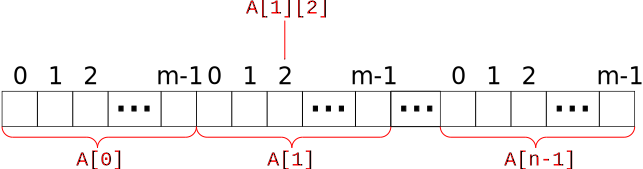
\includegraphics[width=0.65\textwidth]{matrix.pdf}
  \end{center}
  Mátrixok összeadása: $(A+B)[i,j] = A[i,j] + B[i,j]$, ahol $A$ és $B$ két $n\times m$ méretű mátrix.\\
\end{frame}

%25
\begin{frame}
  \begin{exampleblock}{\textattachfile{mtxOsszead1.cpp}{mtxOsszead1.cpp}}
    \scriptsize
    \vspace{-.2cm}
    \lstinputlisting[style=cpp,linerange={5-21},numbers=left,firstnumber=5]{mtxOsszead1.cpp}
    \vspace{-.2cm}
  \end{exampleblock}
\end{frame}

%26
\begin{frame}
  \scriptsize
  \begin{exampleblock}{\textattachfile{mtxOsszead1.cpp}{mtxOsszead1.cpp}}
    \meret{7}
    \vspace{-.2cm}
    \lstinputlisting[style=cpp,linerange={22-42},numbers=left,firstnumber=22]{mtxOsszead1.cpp}
    \vspace{-.2cm}
  \end{exampleblock}
\end{frame}

%27
\begin{frame}[fragile]
  \begin{block}{Kimenet}
    \vspace{-.3cm}
    \begin{verbatim}
11 12 13 14   33 49 36 12   44 61 49 26 
21 22 23 24 + 20 45 24 18 = 41 67 47 42 
31 32 33 34   19 10 11 42   50 42 44 76
\end{verbatim}
    \vspace{-.2cm}
  \end{block}
  \vfill
  Hogyan adható át egy mátrix függvénynek?\\
  \begin{exampleblock}{OK \checkmark}
    \vspace{-.1cm}
    \texttt{void fv(int t[SOROK][OSZLOPOK]) \{ //...\\
    void fv(int t[][OSZLOPOK]) \{ //...\\
    void fv(int (*t)[OSZLOPOK]) \{ //...}
  \end{exampleblock}
  \begin{alertblock}{Hiba X -- Ez mutatótömb, nem mátrix!}
    \vspace{-.1cm}
    \texttt{void fv(int *t[OSZLOPOK]) \{ //...}
  \end{alertblock}
\end{frame}

%28
\begin{frame}
  \begin{exampleblock}{\textattachfile{mtxOsszead2.cpp}{mtxOsszead2.cpp}}
    \lstinputlisting[style=cpp,linerange={44-53},numbers=left,firstnumber=44]{mtxOsszead2.cpp}
  \end{exampleblock}
\end{frame}

%29
\begin{frame}
  \scriptsize
  \begin{exampleblock}{\textattachfile{mtxOsszead2.cpp}{mtxOsszead2.cpp}}
    \meret{7}
    \lstinputlisting[style=cpp,linerange={5-24},numbers=left,firstnumber=5]{mtxOsszead2.cpp}
  \end{exampleblock}
\end{frame}

%30
\begin{frame}
  \scriptsize
  \begin{exampleblock}{\textattachfile{mtxOsszead2.cpp}{mtxOsszead2.cpp}}
    \scriptsize
    \vspace{-.2cm}
    \lstinputlisting[style=cpp,linerange={25-42},numbers=left,firstnumber=25]{mtxOsszead2.cpp}
    \vspace{-.2cm}
  \end{exampleblock}
\end{frame}

%31
\subsection{Dinamikus mátrixok}
\begin{frame}
  \begin{columns}[T]
    \column{.5\textwidth}
      Probléma:
      \begin{itemize}
        \item[] rugalmatlan függvények, mert az oszlopok száma rögzített
      \end{itemize}
      \vfill
      Megoldás:
      \begin{itemize}
        \item hozzunk létre dinamikusan vektorokat (pl. \texttt{int*}-gal címezhetők), majd 
        \item ezek címeit tároljuk egy újabb, dinamikus vektorban (\texttt{int**}, mutatótömb)!
      \end{itemize}
    \column{.5\textwidth}
      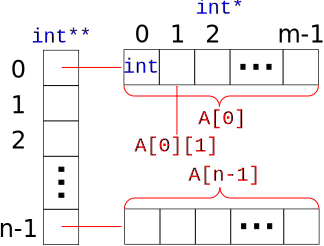
\includegraphics[width=\textwidth]{matrix2.pdf}
  \end{columns}
\end{frame}

%32
\begin{frame}
  \footnotesize
  \begin{exampleblock}{\textattachfile{mtxOsszead3.cpp}{mtxOsszead3.cpp}}
    \vspace{-.2cm}
    \footnotesize
    \lstinputlisting[style=cpp,linerange={56-70},numbers=left,firstnumber=56]{mtxOsszead3.cpp}
    \vspace{-.2cm}
  \end{exampleblock}
\end{frame}

%33
\begin{frame}
  \begin{exampleblock}{\textattachfile{mtxOsszead3.cpp}{mtxOsszead3.cpp}}
    \footnotesize
    \vspace{-.2cm}
    \lstinputlisting[style=cpp,linerange={6-20},numbers=left,firstnumber=6]{mtxOsszead3.cpp}
    \vspace{-.2cm}
  \end{exampleblock}
\end{frame}

%34
\begin{frame}
  \begin{exampleblock}{\textattachfile{mtxOsszead3.cpp}{mtxOsszead3.cpp}}
    \footnotesize
    \vspace{-.2cm}
    \lstinputlisting[style=cpp,linerange={22-29},numbers=left,firstnumber=22]{mtxOsszead3.cpp}
    \lstinputlisting[style=cpp,linerange={49-54},numbers=left,firstnumber=49]{mtxOsszead3.cpp}
    \vspace{-.2cm}
  \end{exampleblock}
\end{frame}

%35
\begin{frame}
  Alternatív megoldás:
  \begin{itemize}
    \item utánozzuk a ``statikus'' tömbök memóriabeli szerkezetét, azaz
    \item valójában vektornak foglalunk helyet, és erre képezzük le a mátrix elemeit
  \end{itemize}
  \begin{center}
    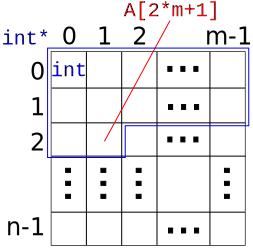
\includegraphics[scale=0.6]{matrix3.pdf}
  \end{center}
\end{frame}

%36
\begin{frame}
  \scriptsize
  \begin{exampleblock}{\textattachfile{mtxOsszead4.cpp}{mtxOsszead4.cpp}}
    \vspace{-.2cm}
    \lstinputlisting[style=cpp,linerange={44-60},numbers=left,firstnumber=44]{mtxOsszead4.cpp}
    \vspace{-.2cm}
  \end{exampleblock}
\end{frame}

%37
\begin{frame}
  \begin{exampleblock}{\textattachfile{mtxOsszead4.cpp}{mtxOsszead4.cpp}}
    \meret{7}
    \lstinputlisting[style=cpp,linerange={6-25},numbers=left,firstnumber=6]{mtxOsszead4.cpp}
  \end{exampleblock}
\end{frame}

\end{document}